%!TEX root = ../crimson_throne_book_main.tex
% 2015-03-28
A set of double doors in the far wall is the only way to continue. Balian pushes open the passage to\hyperref[fig:Temple-of-Urgathoa-Inner-Sanctum-523051443 ]{ the inner sanctum, the heart of the temple's corruption } : a high-domed chamber with six basins lining the walls, containing foul bubbling liquids in distinct blue, green, red, purple, white and brown colors. Each fills the air with its own sharp reek, creating a noxious, eye-watering bouquet. At the room's center, rising from a wide pool of crystalline water, stands a golden statue, depicting a beautiful woman with a lower body of bones. She holds a scythe in her left hand. From the far side of the pool the high priestess of Urgathoa, the haughty Lady Andaisin, greets her visitors: "And so you have finally found your way to the heart of \hyperref[fig:Temple-of-Urgathoa-523050074]{ my temple } , you ignorant fools. Know that you stand in the mighty presence of the architect of your city's demise. You call this a terrible plague, while I know it as the gentle kiss of the Pallid Princess. Yet I am still prepared to show you mercy. Choose one of these colored scourges to become one with the goddess. Those who drink I shall only cripple, leaving you to enjoy the wonder of Urgathoa's gift as it quickens inside your flesh. Those who abstain are fools, not fit to house a divine offering. You may fall at my feet and I shall make your end swift!" \\

\begin{figure}[h]
	\centering
	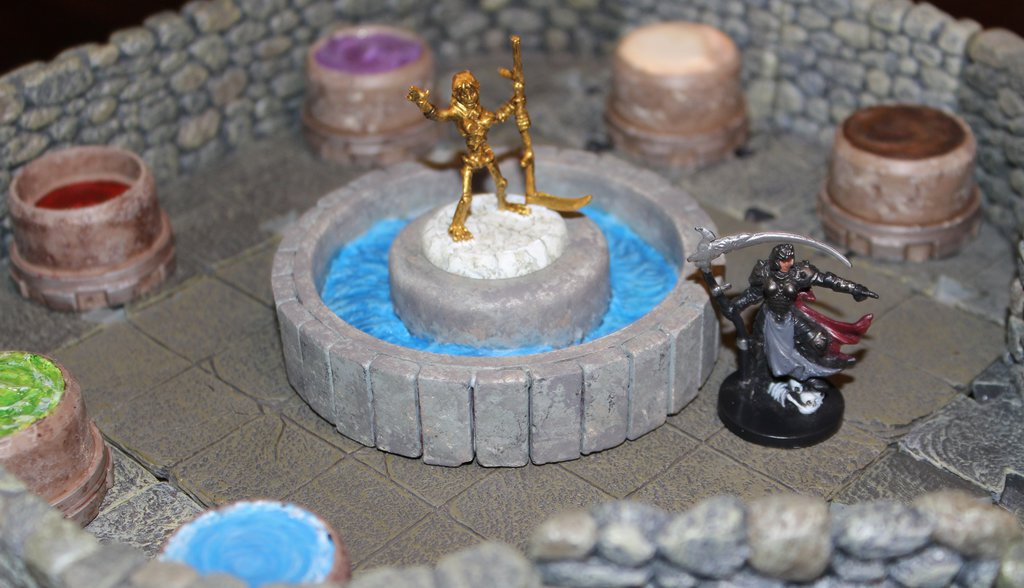
\includegraphics[width=0.39\textwidth]{images/Temple-of-Urgathoa-Inner-Sanctum-523051443 .jpg}
	\caption{Temple of Urgathoa Inner Sanctum}
	\label{fig:Temple-of-Urgathoa-Inner-Sanctum-523051443 }
\end{figure}

\begin{figure}[h]
	\centering
	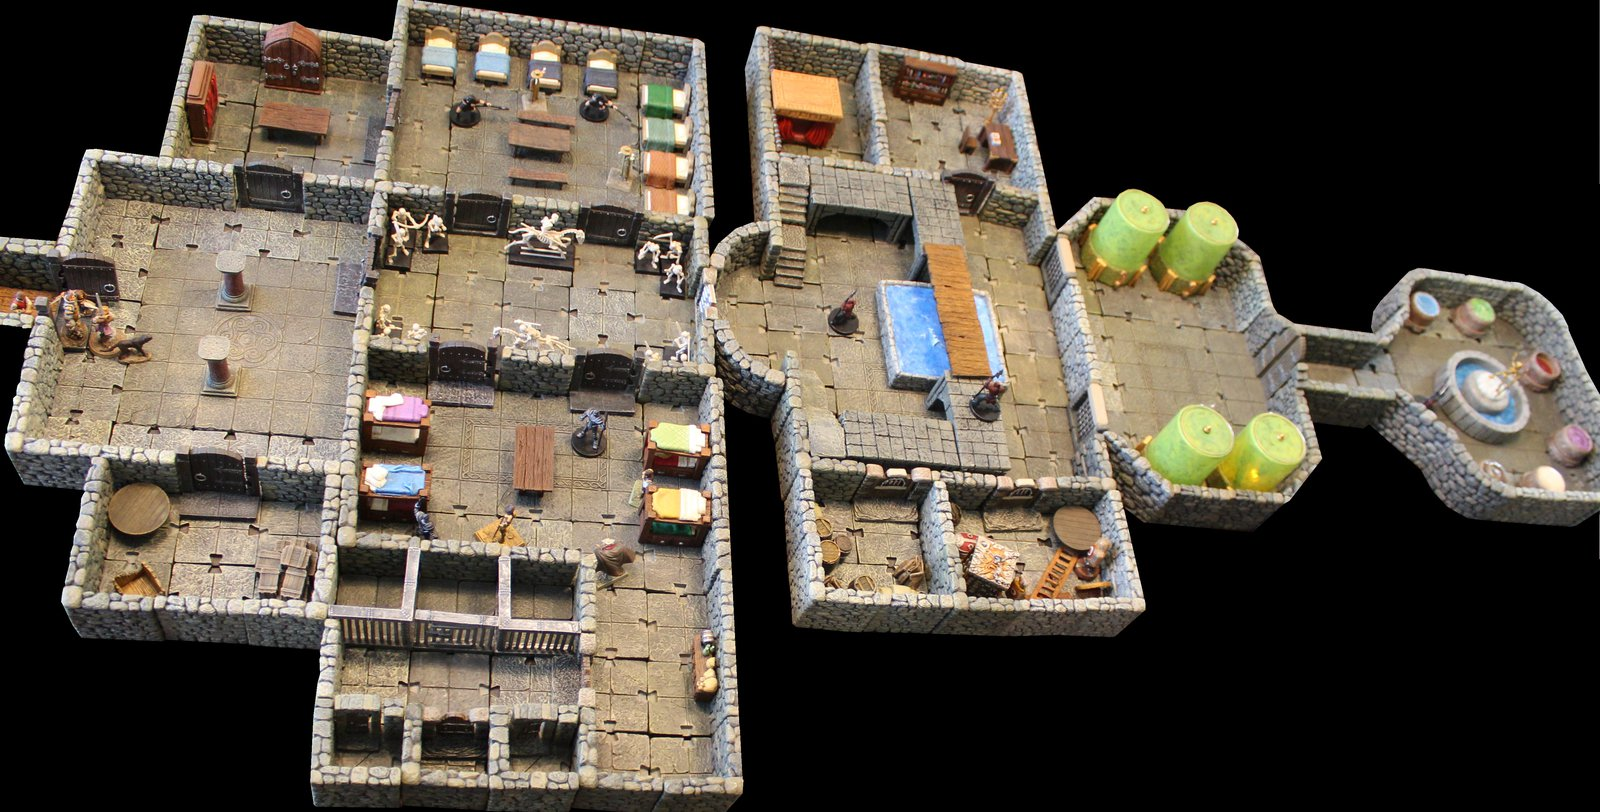
\includegraphics[width=0.39\textwidth]{images/Temple-of-Urgathoa-523050074.jpg}
	\caption{Temple of Urgathoa}
	\label{fig:Temple-of-Urgathoa-523050074}
\end{figure}

Puk is the first to react and rushes into the room, making his way around the pool. He leaves his friends at the entrance, who suddenly see the golden statue come to life and jump down from its stone pedestal in the middle of the pool, landing between them.\hyperref[fig:Statue-of-Urgathoa-attacks-523052019]{ The animated sculpture swings its scythe at Balian } and as she connects with his flesh, the brown pool starts boiling, claiming some of the ranger's strength. Next Lady Andaisin simply steps into the air, as if walking on an invisible set of stairs. Sjo realizes that she is under the effect of an  {\itshape air walk} spell, which will make fighting her very tricky. As he prepares an attempt to counter her flight magic, the priestess calls down a vengeful pillar of fire from her goddess, catching Quint, Sjo, Balian and Spyder in her  {\itshape flame strike} . The Shoanti healer laughs as most of the fire glides off his skin and throws his  {\itshape dispel magic} at the woman, sending her back down to the floor. The companions focus their attacks on the statue first, managing a few deep cuts in her golden skin. Her sharp scythe cleaves through the air with heavy swoops, missing only by a hair's breadth. Puk replies with two biting sneak attacks. Quint trips the thing with his whip, giving Balian the opportunity to finish it off. Meanwhile Sjo tries to keep Lady Andaisin busy. She easily resists his  {\itshape hold person} and prays for another  {\itshape flame strike} on her enemies' heads. Fortunately Balian is the only one who suffers the full effect of the unholy fire. \hyperref[fig:Facing-Lady-Andaisin-523052184]{ The fight now moves to the other side of the pool } , where Lady Andaisin is starting to lose the cocky grin on her face. She takes some heavy damage and, even though she succeeds at taking Puk out of the fight with a  {\itshape blindness} spell, she is sorely pressed. She looks quite proficient with her scythe, but being outnumbered four to one, she does not stand a chance. When she carves into Balian, Spyder reacts furiously and takes her down with his ferocious bite. \\

\begin{figure}[h]
	\centering
	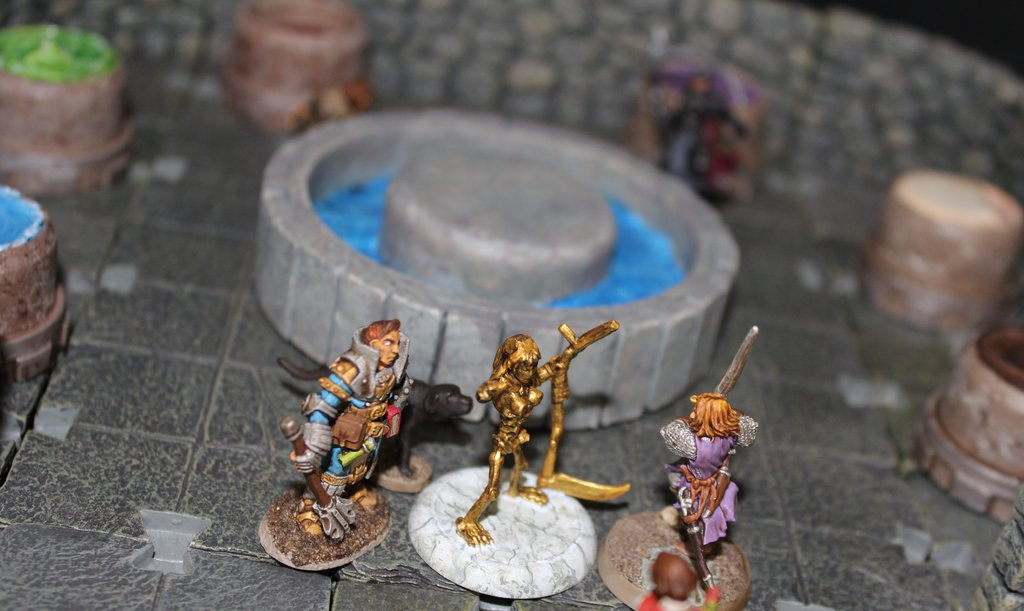
\includegraphics[width=0.39\textwidth]{images/Statue-of-Urgathoa-attacks-523052019.jpg}
	\caption{Statue of Urgathoa attacks}
	\label{fig:Statue-of-Urgathoa-attacks-523052019}
\end{figure}

\begin{figure}[h]
	\centering
	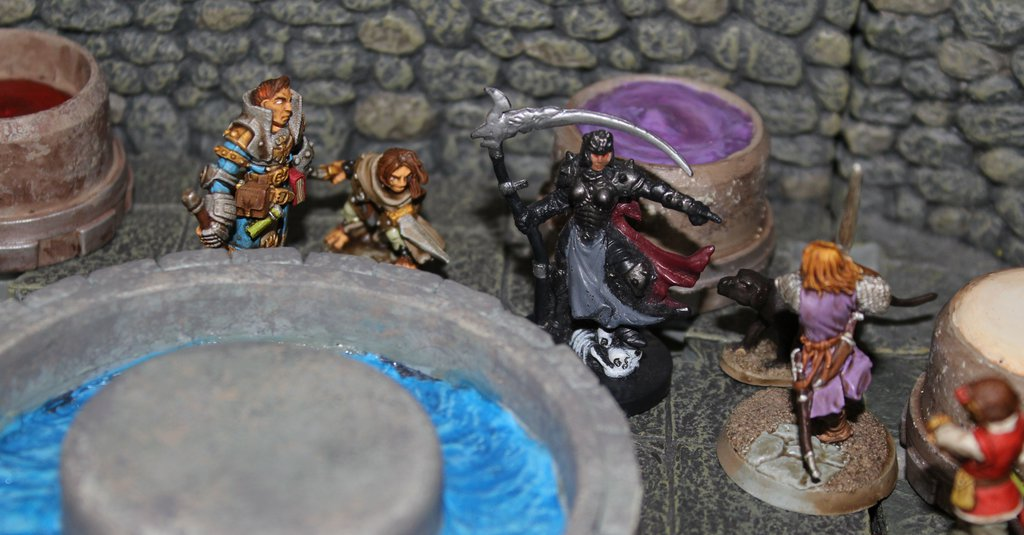
\includegraphics[width=0.39\textwidth]{images/Facing-Lady-Andaisin-523052184.jpg}
	\caption{Facing Lady Andaisin}
	\label{fig:Facing-Lady-Andaisin-523052184}
\end{figure}

A feeling of peace immediately descends upon the room. The colored fluids stop bubbling and the golden statue melts away in vile slime. So much for a well-deserved reward in pure gold, although it looks like Andaisin is wearing some valuable magical items as well. So there still is some nice loot to be divided, albeit that such treasure always comes at a price, literally: ten percent to the city's coffers. Quint gets sick just thinking about it. Still, he feels no qualms when he claims Andaisin's strength and constitution boosting girdle and hands her {\itshape headband of inspired wisdom} to Balian. Sjo is happy to take two powerful wands off Andaisin's dead body: a  {\itshape wand of remove disease} and one of  {\itshape cure serious wounds} . 